\documentclass{summarysheet}

\begin{document}


\maketitle{6}{Batteries and Capacitance}

\begin{multicols}{2}

\begin{topicbox}{Conductors in Electrostatic Equilibrium}

\noindent In a conductor (charged or neutral) that is in \emph{electrostatic equilibrium}, all charges are at rest. This leads to:
\begin{multicols}{2}
\begin{itemize}
\item All excess charge is on the surface.
\item The entire conductor is all at the same potential.
\item The electric field inside is zero.
\item The exterior electric field is perpendicular to the surface.
\item The surface charge density and electric field strength is largest at sharp corners.
\end{itemize}

\includegraphics[scale=0.8]{fig_conductor.pdf}
\end{multicols}
\end{topicbox}


\begin{topicbox}{Batteries}

\noindent Potential difference $\Delta V$ is caused by separation of positive and negative charge. Batteries create separation of charge by chemical reactions; the reactions do \emph{work} on the positive charge to lift them to the positive terminal.
\begin{multicols}{2}
\begin{itemize}
\item The work done per charge is called the emf of the
battery:
\[
\mathcal{E} = W_\text{chem}/q.
\]
\item The charge separation creates a potential difference $\Delta V_\text{bat}$ between the terminals.
\item An ideal battery has $\mathcal{E} = \Delta V_\text{bat}$; for real batteries, $\Delta V_\text{bat} < \mathcal{E}$.
\item For batteries connected in \emph{series} -- positive terminal to negative terminal -- the voltages add.
\end{itemize}
\begin{center}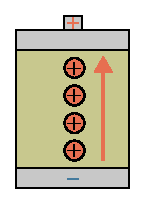
\includegraphics[scale=0.8]{fig_battery.pdf}\end{center}
\end{multicols}

\end{topicbox}







\begin{topicbox}{Energy in a Capacitor}

\noindent Capacitors store an amount of energy given by
\begin{eqbox}
U_\text{C} = \frac{Q^2}{2C} = \frac{1}{2} C \Delta V^2.
\end{eqbox}
This energy can be released very quickly. The energy is actually stored in the electric field, which has an energy density
\[
u_E = \frac{\text{energy stored}}{\text{volume in which it's stored}} = \frac{\epsilon_0}{2} E^2.
\]

\end{topicbox}



\begin{topicbox}{Dielectrics}

\noindent Inserting a dielectric -- a polarized insulator -- into a capacitor creates an induced electric field which reduces the electric field and voltage by an amount $\kappa$, the dielectric constant. This constant varies depending on the dielectric material. The overall effect of the dielectric is to increase the capacitance of the capacitor,
\[
C = \kappa C_0,
\]
where $C_0$ is the vacuum capacitance.
\end{topicbox}



\begin{topicbox}{Capacitors}

\noindent Two equally but oppositely charged conductors form a capacitor. The potential difference $\Delta V$ across the plates of a capacitor is proportional to the charge on each plate $Q$. The proportionality constant is called the \emph{capacitance} $C$:
\[
C = {Q}/{\Delta V}.
\]
The unit of capacitance is the Farad (F): 1 F = 1 C/V.  It’s more useful to turn around the equation above to find the amount of charge on a capacitor:
\begin{eqbox}
Q = C\Delta V.
\end{eqbox}
\end{topicbox}



\begin{topicbox}{The Parallel Plate Capacitor}
\begin{multicols}{2}
\noindent For a capacitor made from two parallel plates of area $A$ and separated by distance $d$, the potential difference and electric field are related by
\begin{eqbox}
\Delta V_\text{C} = Ed.
\end{eqbox}
\noindent The \emph{capacitance} is given by
\begin{eqbox}
C = \epsilon_0 A / d.
\end{eqbox}
\begin{center}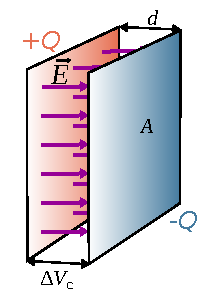
\includegraphics[scale=0.8]{fig_cap2.pdf}\end{center}
\end{multicols}
\end{topicbox}




\begin{topicbox}{Batteries and Capacitors}
\begin{multicols}{2}
\noindent A capacitor is charged by connecting it to a battery, which does work on the charge in the battery, moving it to the capacitor plate. This drives a current, in which charges flow along the wire to the capacitor. This current continues until the potential difference of the capacitor is equal to that of the battery. More than one capacitor can be connected to a battery. Two possible connections are \emph{parallel} and \emph{series}.

\begin{center}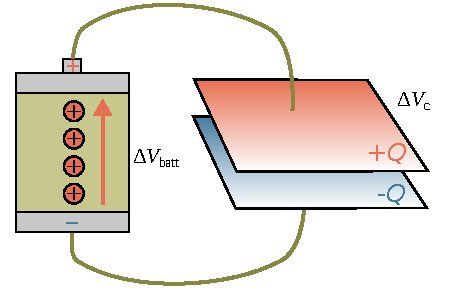
\includegraphics[scale=0.65]{fig_cap_batt.pdf}\end{center}
\end{multicols}

\begin{multicols}{2}
\noindent \textbf{Capacitors in Parallel}
%\begin{multicols}{2}
\noindent When connected in parallel, capacitors have the same voltage $\Delta V_\text{C}$ but different charge. Capacitors add to an \emph{equivalent capacitance}:
\begin{eqbox}
C_\text{eq} = C_1 + C_2 + C_3 + \cdots
\end{eqbox}
\begin{center}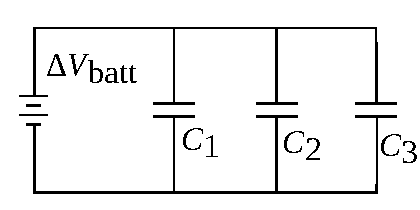
\includegraphics[scale=0.5]{fig_cap_circuit.pdf}\end{center}
%\end{multicols}

\vspace{0.2in}

\noindent \textbf{Capacitors in Series}
%\begin{multicols}{2}
\noindent When connected in series, capacitors have the same charge $Q$ but different voltages. Capacitors add in inverse:
\begin{eqbox}
C_\text{eq} = \left( \frac{1}{C_1} + \frac{1}{C_2}  + \cdots \right)^{-1}.
\end{eqbox}
\begin{center}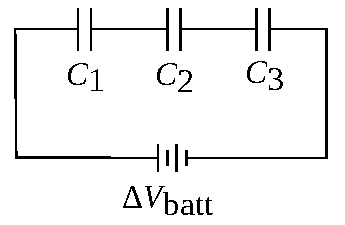
\includegraphics[scale=0.5]{fig_cap_circuit2.pdf}\end{center}
\end{multicols}

\end{topicbox}








\end{multicols}





\makebanner{Electricity and Magnetism}

\end{document}



